\section{Experiment}
\label{sec:experiment}

In this section, we will establish real-world comparison with human baselines. We will also investigate the effect of varies components in our pipeline, including visual randomization, staged reset, and fine-tuning.

\subsection{Surpassing Human-Teleop Baseline}

\begin{figure}
    \centering
    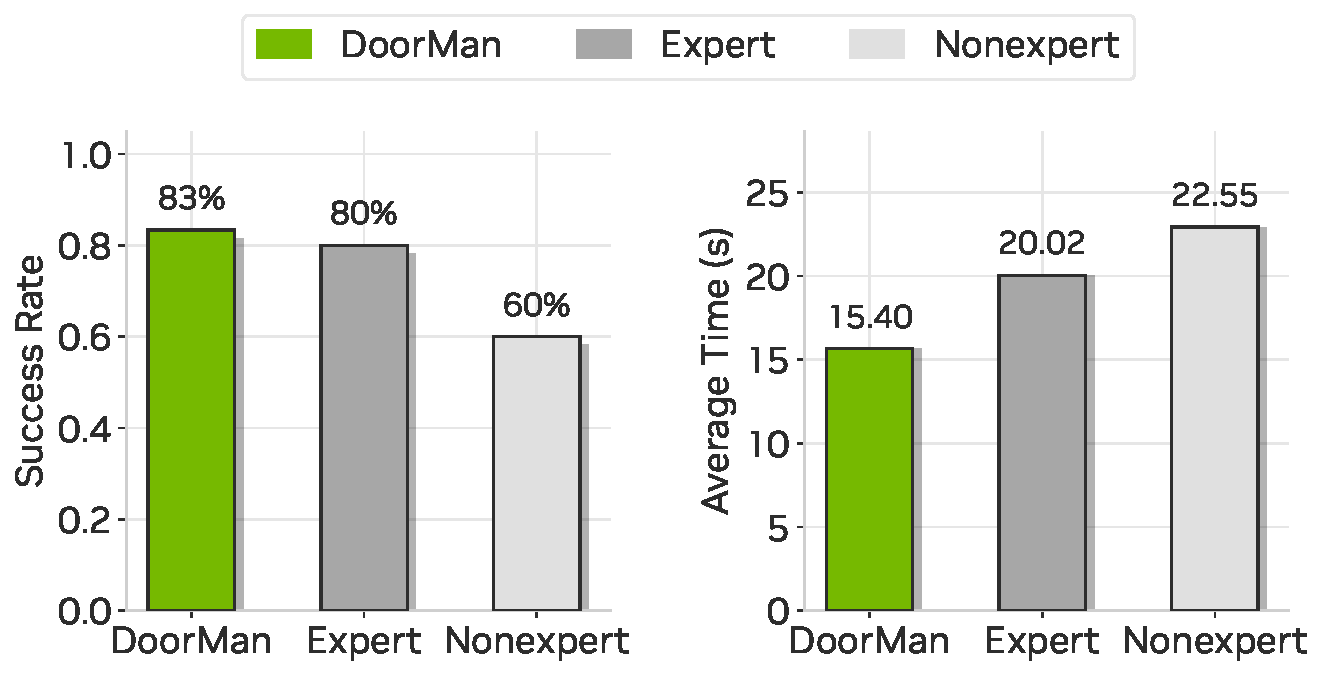
\includegraphics[width=0.65\linewidth]{figs/real-world-door-compare.pdf}
    \caption{Average performance on all door opening tasks. Left: success rate (the higher the better). Right: task fluency in terms of time taken to complete the door opening task (the lower the better).}
    \label{fig:performance}
\end{figure}

The main question of this work is whether RGB sim-to-real RL can address the long-lasting problem of humanoid door-opening in the wild beyond pure behavioral cloning, whose upper bound is determined by human teleoperation data quality. We hypothesize that the current whole-body teleoperation technology, due to its unintuitive nature, create a gap in both efficiency and success rate compared to direct human operation, and that RGB sim-to-real RL offers better performance.

\minisection{Scenario Setups} We set up evaluation scenarios in both simulation and real world. Three door categories are used:

\begin{itemize}
    \item Rotational handle, opening into the direction of travel \textbf{(push lever)}: the simplest task.
    \item Rotational handle, opening against the direction of travel \textbf{(pull lever)}: requiring skillful manipulation in constrained space and long-horizon behavior.
    \item Push-bar handle, opening into the direction of travel \textbf{(push bar)}: requiring forceful interaction to overcome the spring-loaded hinge.
\end{itemize}

In evaluation, simulation visuals are randomized from textures in a holdout set. Real-world visuals are unseen during training.

In all experiments, the robot is randomly placed to be 1 meter in front of the door and facing the center of the door. Yaw orientation is perturbed by a uniform range of $\pm 0.3$ radians. Success rate and completion time are evaluated at when the robot traverses through the door and reaches a point 1 m beyond the door frame on the opposite side.

\minisection{Human Teleop Baseline} Human teleoperators use the same whole-body controller~\citep{ben2025homie} as the autonomous policy. The teleoperator wears a VR headset with joysticks to control the robot via inverse kinematics, details of which can be found in Appendix \ref{app:teleop}. Teleoperators are classified as \textbf{non-experts} (with less than 1 day of experience teleoperating robots), or \textbf{experts} (with more than 3 months of full-time experience).

Figure \ref{fig:performance} shows that \method{} performs on par in the real world with an expert teleoperator in terms of success rate while being 28\% better than non-experts. In addition, \method{} shines in terms of task fluency, outperforming experts by 23.8\% and non-experts by 31.7\%. Qualitatively, teleoperators often fail to gauge the spring-loaded force of the door handle and the door hinge, or whether the robot is leaning with the appropriate amount to maintain smooth and consistent opening speed. They also often fail to track the revolving path of the swinging door, highlighting a unique challenge in manipulating articulated objects under kinematic constraints, which requires the policy to be aware and compliant of such constraints and maintain whole-body balance at the same time. The feedback information needed for this behavior is beyond the current generation of VR teleoperation, but learnable interactively in simulation.

\subsection{Effect of Photorealistic Visual Randomization}

\textit{How does photorealistic randomization quantitatively affect the generalization on unseen visual features?} We design an ablation study on the visual diversity during training, starting with no visual randomization, where objects are coated in a default gray reflective color, preserving the geometries without textures. We then add 10\% or 100\% of all PBR materials available in randomization, coupled with an additional condition that toggles dome-light randomization to vary lighting and environmental appearance.

Table \ref{tab:vis-rand-ablation} shows that using all available texture and dome light during training yields the best generalization capability in unseen scenarios, with 81-86\% success rates on respective sub-tasks. Removing dome light randomization, and hence the randomization in lighting condition, results in 15-30\% performance drop, with the most significant effect on pulling doors with lever handles, which is the most long-horizon and challenging task. We also observe that with 10\% of all textures available, we can already achieve comparable performance with using 100\%, with only 4-8\% performance drop. Using no visual feature randomization, however, reduces the task success rates to 5-20\%, confirming the effectiveness of texture and lighting randomization in helping sim-to-real policies generalize. We additionally run a setting with only randomizing with solid color materials, paired with dome light randomization, which corresponds to settings in earlier RGB sim-to-real works such as~\citet{tobin2017domain,zhu2018reinforcement}. This setting achieves a commendable success rate of 65.8-70\%. This remaining gap reflects the advantage of modern high-fidelity rendering, which provides richer material and lighting variation and thus stronger visual generalization.

% \begin{itemize}
%     \item No-randomization: objects are coated in a default dark-grey color, preserving the geometries without textures.
%     \item solid-color texture, with dome-light randomization
%     \item 10\% texture, no dome-light randomization
%     \item 10\% texture, with dome-light randomization
%     \item 100\% texture, no dome-light randomization
%     \item 100\% texture, with dome-light randomization
% \end{itemize}

% \begin{table}[]
% \begin{tabular}{@{}lccc@{}}
% \toprule
%                                                                                 & \textbf{\begin{tabular}[c]{@{}c@{}}Push\\ Lever\end{tabular}} & \textbf{\begin{tabular}[c]{@{}c@{}}Pull\\ Lever\end{tabular}} & \textbf{Push Bar} \\ \midrule
% \textbf{No Randomization}                                                       & 10.8                                                          & 5.0                                                           & 20.0              \\ \midrule
% \textbf{\begin{tabular}[c]{@{}l@{}}Solid Color\\ + Dome Light\end{tabular}}     & 67.5                                                          & 65.8                                                          & 70.0              \\ \midrule
% \textbf{\begin{tabular}[c]{@{}l@{}}10\% Texture\\  w/o Dome Light\end{tabular}} & 58.3                                                          & 50.8                                                          & 76.7              \\ \midrule
% \textbf{\begin{tabular}[c]{@{}l@{}}10\% Texture\\ + Dome Light\end{tabular}}    & 79.2                                                          & 77.5                                                          & 77.5              \\ \midrule
% \textbf{\begin{tabular}[c]{@{}l@{}}100\% Texture\\ w/o Dome Light\end{tabular}} & 73.3                                                          & 55.8                                                          & 76.7              \\ \midrule
% \textbf{\begin{tabular}[c]{@{}l@{}}100\% Texture\\ + Dome Light\end{tabular}}   & \textbf{85.8}                                                 & \textbf{80.8}                                                 & \textbf{85.0}     \\ \bottomrule
% \end{tabular}
% \caption{Success rates under various visual diversity settings. Models are evaluated out of 120 trials on randomized doors with unseen visual features. \haoru{re-work the visuals}}
% \label{tab:vis-rand-ablation}
% \end{table}

% \begin{table}[t]
% \centering
% \footnotesize
% \setlength{\tabcolsep}{3pt}  % tighter columns
% \begin{tabularx}{\columnwidth}{@{}lccccc@{}}
% \toprule
% \textbf{Setting} &
% \textbf{Texture} &
% \textbf{\makecell{Dome\\Light}} &
% \textbf{\makecell{Push\\Lever}} &
% \textbf{\makecell{Pull\\Lever}} &
% \textbf{\makecell{Push\\Bar}} \\
% \midrule
% No Randomization               & ✗ & ✗ & 10.8 & 5.0  & 20.0 \\
% Solid Color + Dome Light       & ✗ & ✓ & 67.5 & 65.8 & 70.0 \\
% 10\% Texture, w/o Dome Light   & 10\% ✓ & ✗ & 58.3 & 50.8 & 76.7 \\
% 10\% Texture, + Dome Light     & 10\% ✓ & ✓ & 79.2 & 77.5 & 77.5 \\
% 100\% Texture, w/o Dome Light  & 100\% ✓ & ✗ & 73.3 & 55.8 & 76.7 \\
% \rowcolor{gray!10}
% \textbf{100\% Texture, + Dome Light} & \textbf{100\% ✓} & \textbf{✓} & \textbf{85.8} & \textbf{80.8} & \textbf{85.0} \\
% \bottomrule
% \end{tabularx}
% \caption{Success rates (\%) under different visual randomization settings. Texture and lighting factors are indicated with ✓ (enabled) or ✗ (disabled). Each configuration is evaluated on 120 unseen-door trials.}
% \label{tab:vis-rand-ablation}
% \end{table}

\begin{table*}[t]
\centering
\small
\arrayrulecolor{nvidiagreen}
\setlength{\tabcolsep}{8pt} 

\begin{tabular}{c l c c c c}
\toprule
\textbf{Experiment} & \textbf{Appearance} & \textbf{DL} &
\textbf{Push Lever} &
\textbf{Pull Lever} &
\textbf{Push Bar} \\
\midrule
1 & No Rand.                 & \xmark & 10.8 &  5.0 & 20.0 \\
2 & Solid-color Rand.        & \cmark & 67.5 & 65.8 & 70.0 \\
3 & +10\% Texture Rand.      & \xmark & 58.3 & 50.8 & 76.7 \\
4 & +10\% Texture Rand.      & \cmark & 79.2 & 77.5 & 77.5 \\
5 & +100\% Texture Rand.     & \xmark & 73.3 & 55.8 & 76.7 \\
\rowcolor{bestrow}
\textbf{6} & \textbf{+100\% Texture Rand.} & \textbf{\cmark} &
\textbf{85.8} & \textbf{80.8} & \textbf{85.0} \\
\bottomrule
\end{tabular}

\caption{Success rates (\%) under visual randomization settings.
\emph{Appearance} denotes the type of visual variation:
\emph{Solid-color Rand.} means uniform recoloring without textures;
\emph{+10\%/100\% Texture Rand.} means percentage of texture randomization.
\emph{DL} indicates dome lighting randomization (\cmark{} enabled, \xmark{} disabled).
Each configuration (Experiment~1–6) is evaluated on 120 unseen-door trials.}
\label{tab:vis-rand-ablation}
\end{table*}



\subsection{Performance Boost in GRPO Fine-Tuning}

% \begin{figure}
%     \centering
%     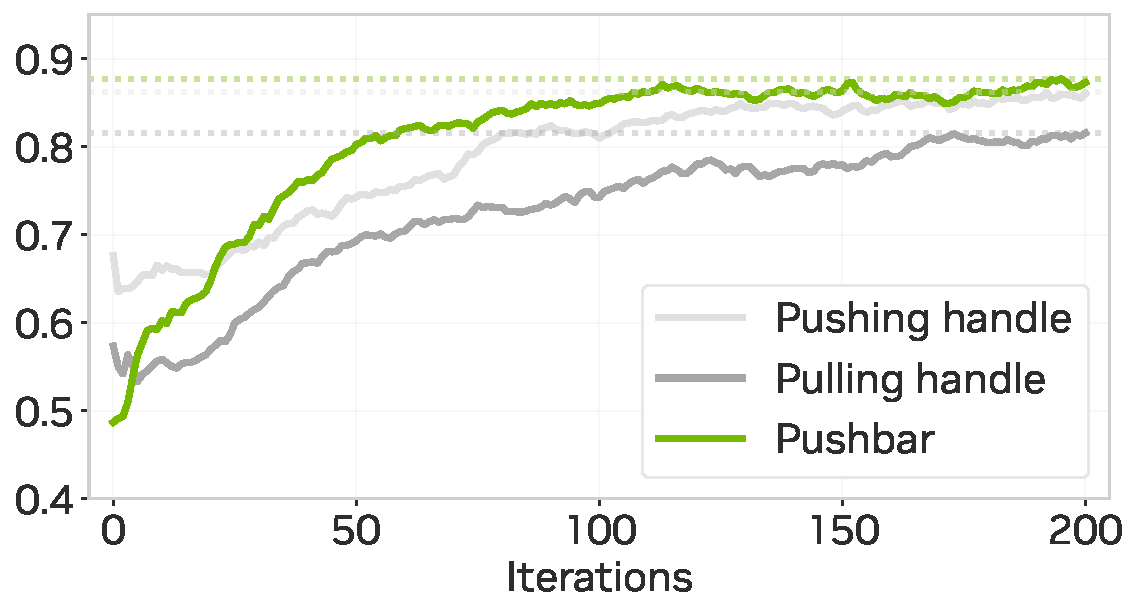
\includegraphics[width=0.5\linewidth]{figs/GRPO_success_rate.pdf}
%     \caption{Training progress of student policy bootstrapping with improvements in task success rate. The dashed lines are teacher policy success rates.}
%     \label{fig:reinforce}
% \end{figure}

\begin{figure}[t]
    \centering
    \begin{subfigure}[b]{0.48\linewidth}
        \centering
        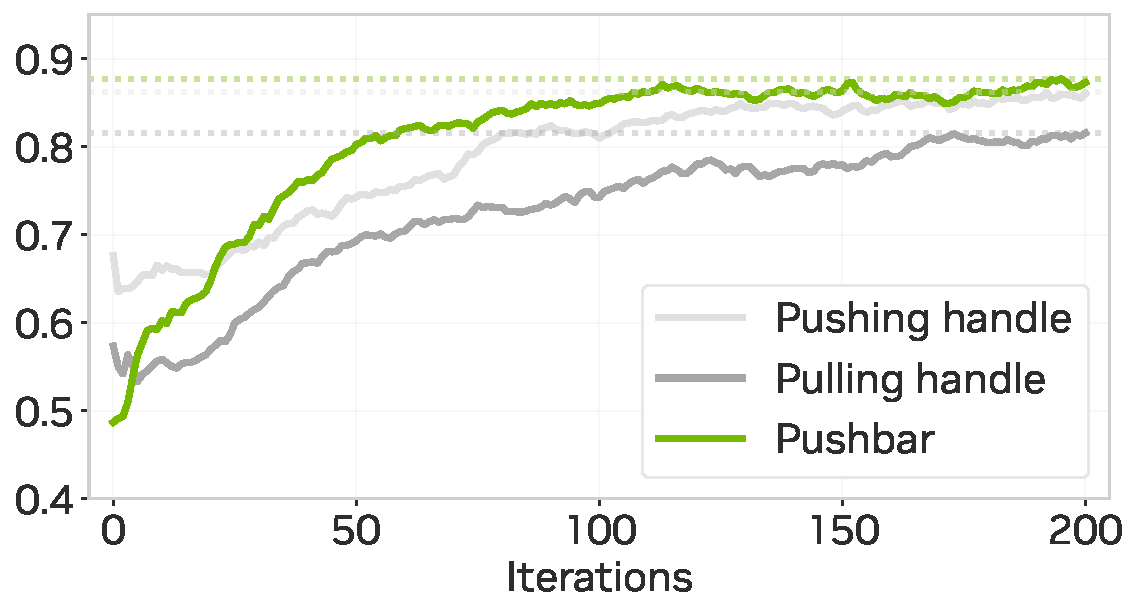
\includegraphics[width=\linewidth]{figs/GRPO_success_rate.pdf}
        \caption{Student policy success rate during GRPO training. 
        Dashed lines show teacher success.}
        \label{fig:reinforce}
    \end{subfigure}
    \hfill
    \begin{subfigure}[b]{0.48\linewidth}
        \centering
        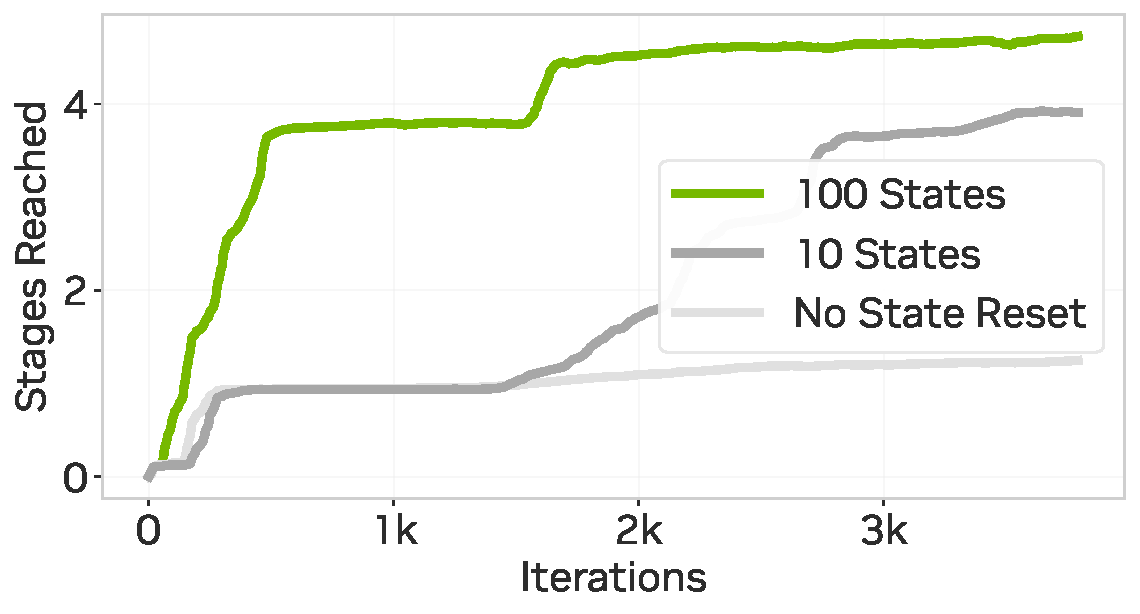
\includegraphics[width=\linewidth]{figs/stage_reached.pdf}
        \caption{Teacher training progress with reset buffer sizes 0, 10, and 100.}
        \label{fig:staged_reset_ablation}
    \end{subfigure}

    \caption{DoorMan training progress: (a) student GRPO bootstrapping and (b) teacher exploration under different staged-reset buffer sizes.}
    \label{fig:training_progress}
\end{figure}

Figure \ref{fig:reinforce} illustrates the progression of the GRPO bootstrapping phase on 3 door-opening sub-tasks. When teacher policies can consistently achieve 80-90\% success rate, the initial student policy performance stales at 50-70\%, suggesting a non-recoverable observability gap. At the end of the bootstrapping, the student policies achieve 80.8-85.8\% sub-task success rates. Across all open door tasks, the improvement curves exhibit a clear plateau that aligns with the teacher upper bound, indicating that GRPO effectively reduces the gap caused by partial observability and serves as a reliable fine-tuning method for humanoid whole body control.

\subsection{Effect of Staged Reset Exploration}

Finally, we run an ablation study to investigate the effect of staged reset exploration on the stability of teacher training. We use a different set of reset buffer sizes of 0, 10, and 100. A buffer size of 10, for example, stores the ten most recent snapshots of the simulation state when an environment enters a stage. Reward tunings are kept consistent in all trials, and the staged reset exploration is not involved in the reward computation at all. Figure~\ref{fig:staged_reset_ablation} shows that with a buffer size of 100, the teacher rapidly reaches most stages within 500 iterations and all stages by roughly 1700 iterations. With a buffer size of 10, it takes over 4000 iterations for the exploration to finish. The exploration fails when not using the reset buffer, as the policy finds it difficult to enter stage 2 (grasping door handle), which is challenging for incurring additional collision penalties when the policy initially fails to skillfully grasp and rotate the door handle, resulting in ``unlearning'' or avoiding entering into this stage.

% \begin{figure}
%     \centering
%     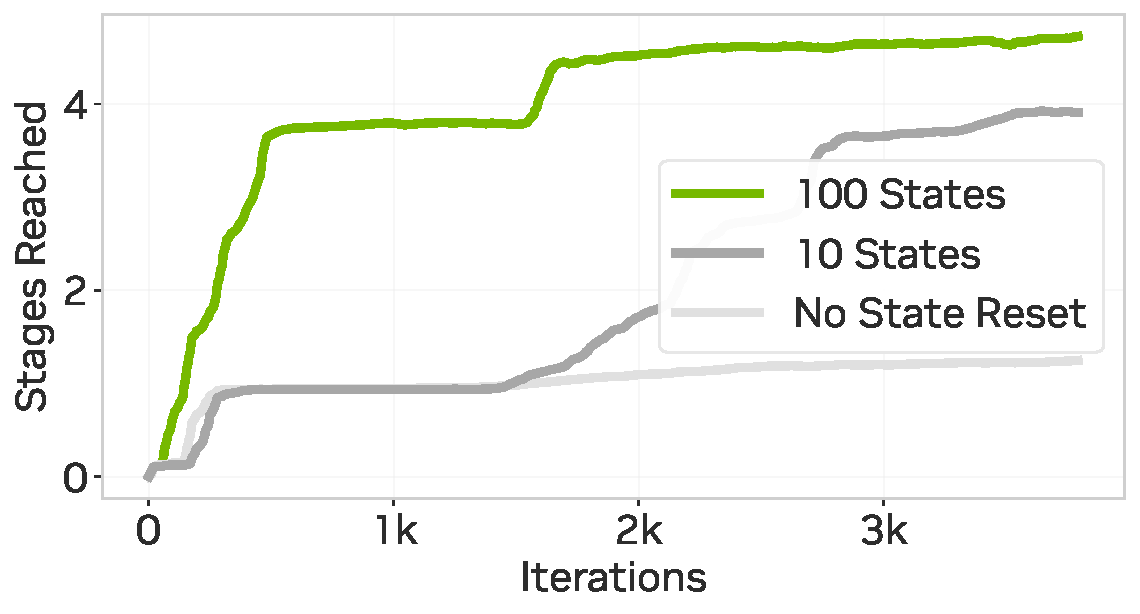
\includegraphics[width=0.5\linewidth]{figs/stage_reached.pdf}
%     \caption{Teacher training progress with different reset buffer sizes of 0, 10 and 100.}
%     \label{fig:staged_reset_ablation}
% \end{figure}